\documentclass[11pt,a4paper]{article}
\usepackage{fontspec}
\usepackage[margin=1.5cm]{geometry}
\usepackage{graphicx}
\usepackage{xcolor}
\usepackage{tabularx}
\usepackage{booktabs}
\usepackage{enumitem}

\definecolor{navy}{HTML}{060C1A}
\definecolor{gold}{HTML}{C5A059}
\definecolor{primary}{HTML}{0284C7}
\definecolor{dark}{HTML}{0F172A}
\definecolor{redalert}{HTML}{DC2626}
\definecolor{graytext}{HTML}{475569}

\pagestyle{plain}

\begin{document}

% ============================================================
% TRANG BÌA
% ============================================================
\begin{center}
    \vspace*{0.5cm}
    {\Huge\bfseries\color{navy} ĐẤU TRƯỜNG OLYMQUIZ ARENA}\\[0.3cm]
    {\LARGE\bfseries\color{primary} CẨM NANG HƯỚNG DẪN SỬ DỤNG VẬN HÀNH TRẬN ĐẤU}\\[0.3cm]
    {\large\bfseries\color{gold} Trình Bày Chi Tiết 13 Màn Hình Thực Tế -- Tiếng Việt Đầy Đủ Dễ Hiểu}\\[0.2cm]
    \rule{\textwidth}{1.5pt}
    \vspace{0.3cm}
    {\small Dành cho Ban Giám Khảo, Thư Ký \& 4 Bạn Thí Sinh Tham Gia Tranh Tài}
    \vspace{0.5cm}
\end{center}

\noindent\textbf{\large QUY TRÌNH 3 BƯỚC ĐIỀU HÀNH DỄ NHỚ CHO BAN GIÁM KHẢO:}\\
\begin{enumerate}[leftmargin=*,itemsep=4pt]
    \item \textbf{Bước 1 (Chuẩn bị)}: Mở trang \texttt{/admin/players} $\rightarrow$ Bấm nút \textbf{[SAO CHÉP LINK THI ĐẤU]} gửi link phòng thi kèm mã PIN (1111, 2222, 3333, 4444) cho 4 bạn thí sinh.
    \item \textbf{Bước 2 (Trong trận)}: Mở bàn \texttt{/admin/live} $\rightarrow$ Nhấn phím \textbf{Space} (Bắt đầu đếm giờ) $\rightarrow$ Hết giờ bấm \textbf{Mở Đáp Án} $\rightarrow$ Nhấn phím \textbf{G} (Chấm điểm tự động).
    \item \textbf{Bước 3 (Bế mạc)}: Sau khi xong 4 vòng $\rightarrow$ Bấm nút \textbf{[4. Bảng Vàng Trao Giải]} để máy chiếu vinh danh Quán quân cùng pháo hoa giấy!
\end{enumerate}

\vspace{0.4cm}
\hrule
\vspace{0.6cm}

% ============================================================
% MÀN HÌNH 1: QUẢN LÝ THÍ SINH
% ============================================================
\noindent{\Large\bfseries\color{primary} MÀN HÌNH 1: QUẢN LÝ 4 THÍ SINH \& CẤP MÃ BẢO MẬT PIN}\\[0.1cm]
\noindent\textit{Địa chỉ truy cập: \texttt{/admin/players} | Người thực hiện: Ban Tổ Chức / Giám Khảo}\\[0.2cm]
\textbf{Mục đích}: Đây là màn hình chuẩn bị đầu tiên trước khi trận đấu chính thức diễn ra.
\begin{itemize}[leftmargin=*,itemsep=2pt]
    \item \textbf{Nút màu xanh [SAO CHÉP LINK THI ĐẤU]}: Bấm nút này để tự động copy toàn bộ đường link bục đấu kèm mã PIN gửi qua Zalo hoặc tin nhắn cho từng bạn thí sinh.
    \item \textbf{Khung Mã PIN (1111, 2222, 3333, 4444)}: Mỗi bục máy có 1 mã bảo mật riêng để chống người lạ vào nhầm bục đấu.
    \item \textbf{Bộ 3 Nút Reset Tổng (Góc trên bên phải)}:
    \begin{itemize}[itemsep=1pt]
        \item \textbf{[Reset Điểm Về 0]}: Đưa điểm số của 4 thí sinh về số 0 trước trận đấu.
        \item \textbf{[Tạo Mới 4 Mã PIN]}: Đổi mã PIN ngẫu nhiên mới và vô hiệu hóa mã cũ.
        \item \textbf{[Reset Cả 4 Bục Máy]}: Xóa trắng toàn bộ thông tin để chuẩn bị cho trận đấu mới.
    \end{itemize}
\end{itemize}

\begin{center}
    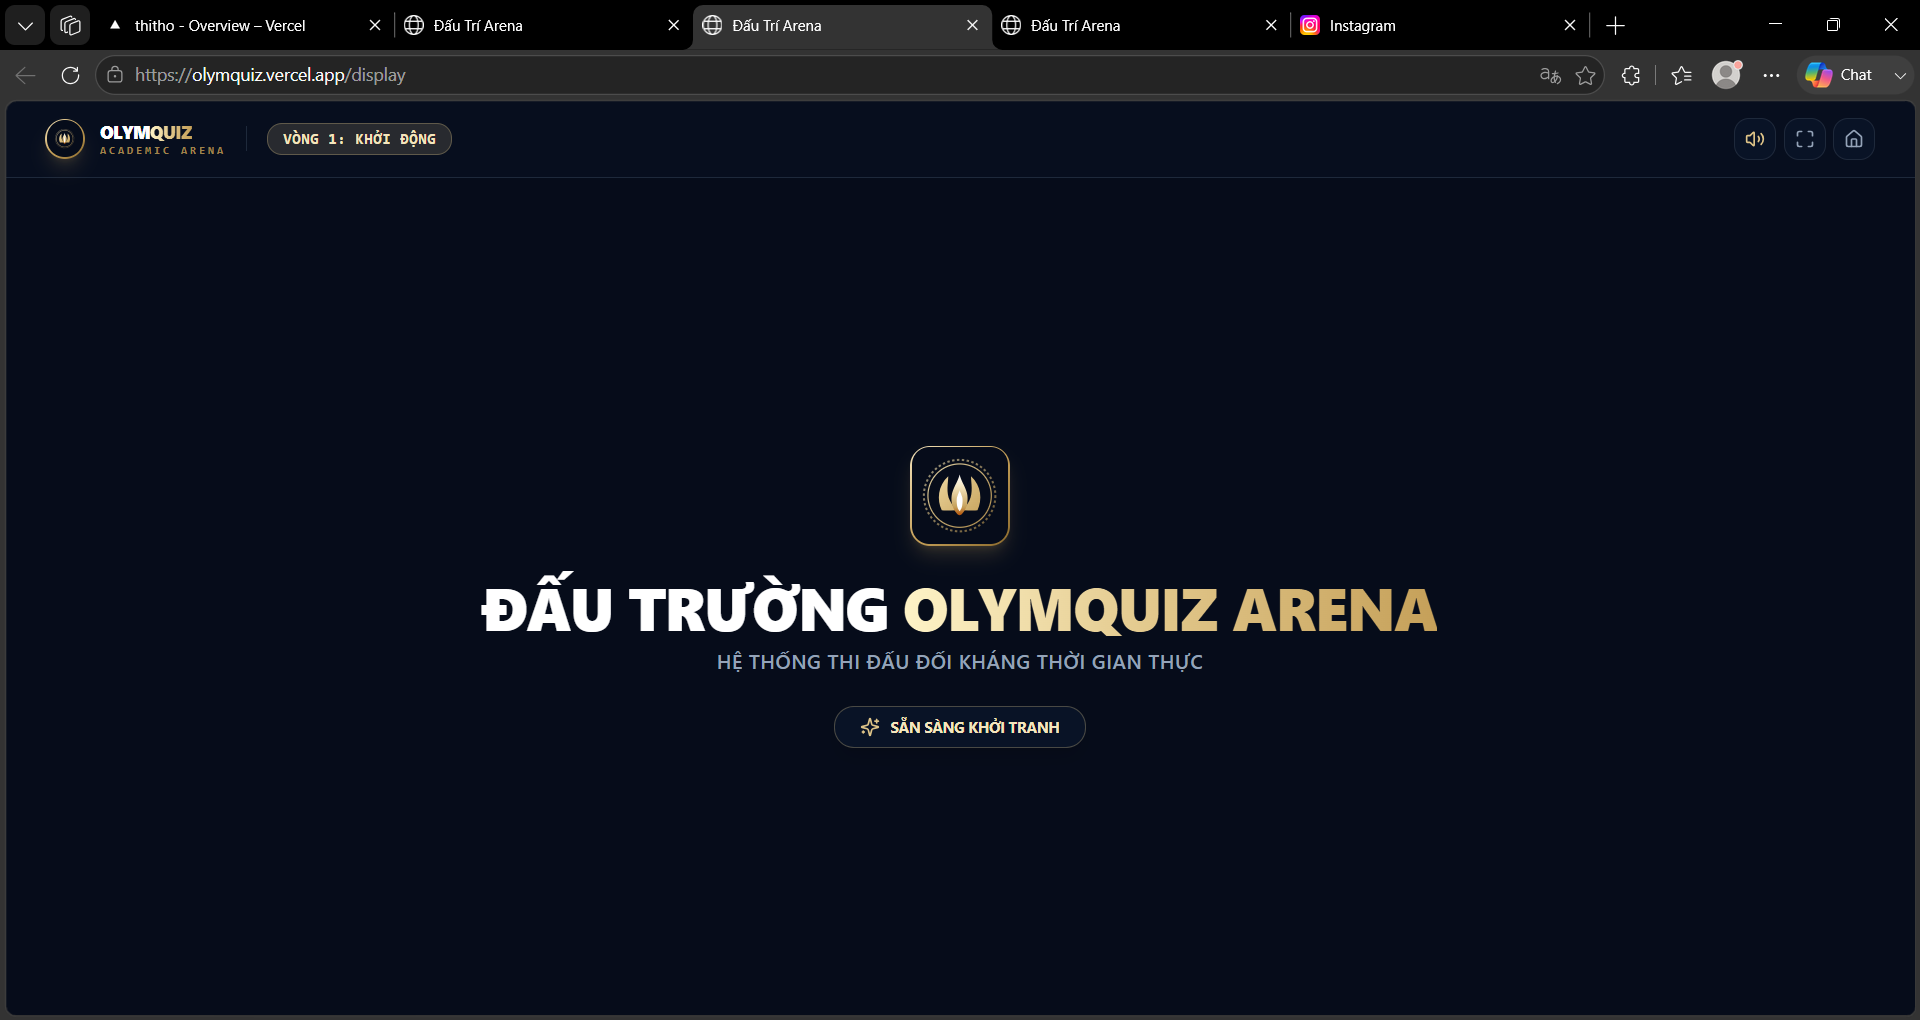
\includegraphics[width=0.96\textwidth]{screenshots/12_admin_players.png}
\end{center}

\newpage

% ============================================================
% MÀN HÌNH 2: THÍ SINH NHẬP PIN
% ============================================================
\noindent{\Large\bfseries\color{primary} MÀN HÌNH 2: THÍ SINH NHẬP MÃ PIN ĐỂ VÀO PHÒNG THI}\\[0.1cm]
\noindent\textit{Địa chỉ truy cập: \texttt{/player/1} đến \texttt{/player/4} | Người thực hiện: Thí Sinh}\\[0.2cm]
\textbf{Mục đích}: Giúp thí sinh đăng nhập an toàn vào đúng bục máy thi đấu của mình.
\begin{itemize}[leftmargin=*,itemsep=2pt]
    \item Thí sinh mở link do Giám Khảo gửi trên điện thoại hoặc máy tính cá nhân.
    \item Gõ mã PIN 4 chữ số (ví dụ: \texttt{1111}) vào ô $\rightarrow$ Bấm nút \textbf{[XÁC NHẬN VÀO PHÒNG THI]}.
    \item Sau khi nhập đúng, bục máy sẽ mở ra giao diện thi đấu trực tiếp.
\end{itemize}

\begin{center}
    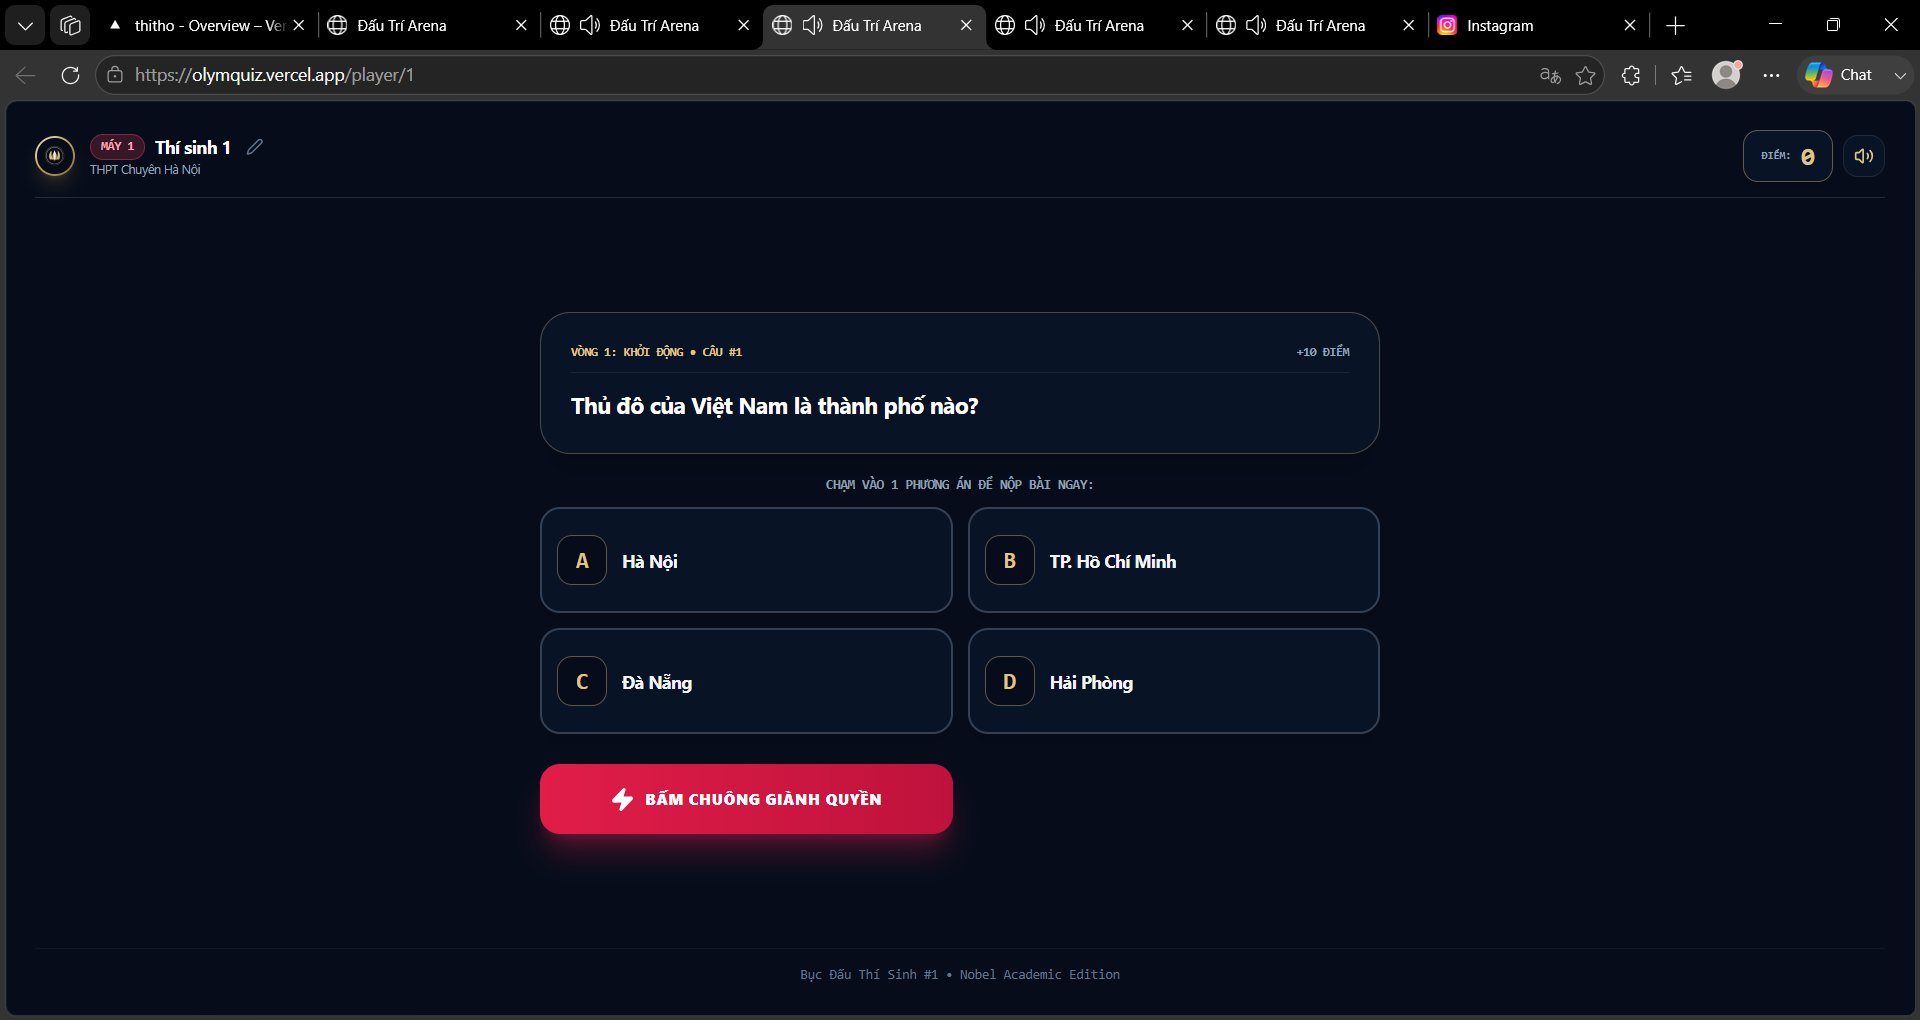
\includegraphics[width=0.96\textwidth]{screenshots/01_login_pin.png}
\end{center}

\vspace{0.4cm}

% ============================================================
% MÀN HÌNH 3: GIAO DIỆN BỤC THÍ SINH
% ============================================================
\noindent{\Large\bfseries\color{primary} MÀN HÌNH 3: GIAO DIỆN THI ĐẤU TRÊN BỤC CỦA THÍ SINH}\\[0.1cm]
\noindent\textit{Địa chỉ truy cập: \texttt{/player/[slot]} | Người thực hiện: Thí Sinh}\\[0.2cm]
\textbf{Mục đích}: Nơi thí sinh đọc câu hỏi và thao tác trả lời trong suốt 4 vòng thi.
\begin{itemize}[leftmargin=*,itemsep=2pt]
    \item \textbf{4 Thẻ Trắc Nghiệm To (A, B, C, D)}: Thí sinh chỉ cần \textbf{chạm 1 lần vào ô đáp án muốn chọn}. Màn hình sẽ đổi sang màu xanh ngọc xác nhận nộp bài thành công kèm thời gian nộp (tính bằng mili-giây).
    \item \textbf{Tự luận \& Ô chữ (Vòng 2)}: Gõ chữ vào ô nhập và bấm nút \textbf{[Nộp Bài]}.
    \item \textbf{Bấm Chuông Cướp Điểm (Vòng 4)}: Nút chuông đỏ to sẽ sáng lên khi có câu cướp điểm, ai bấm nhanh nhất sẽ giành quyền trả lời.
\end{itemize}

\begin{center}
    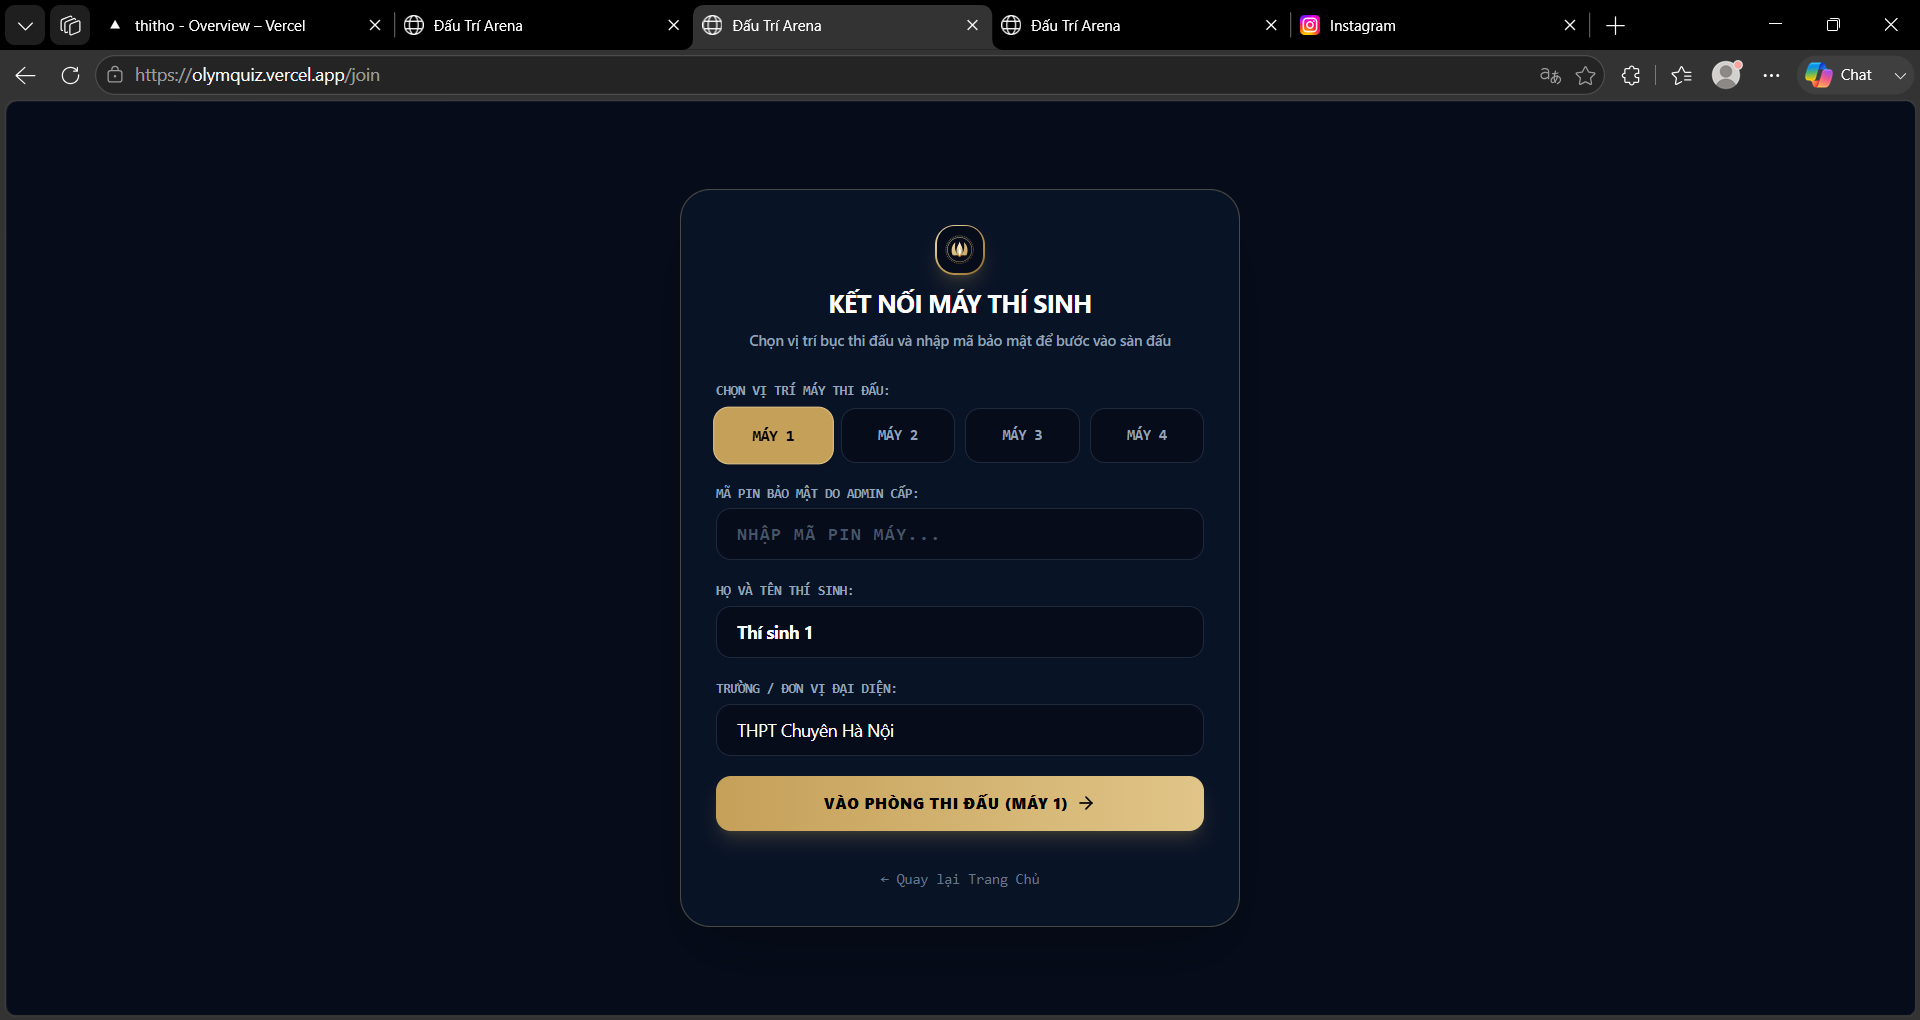
\includegraphics[width=0.96\textwidth]{screenshots/11_player_screen.png}
\end{center}

\newpage

% ============================================================
% MÀN HÌNH 4: BÀN GIÁM KHẢO LIVE
% ============================================================
\noindent{\Large\bfseries\color{primary} MÀN HÌNH 4: BÀN ĐIỀU HÀNH BAN GIÁM KHẢO LIVE}\\[0.1cm]
\noindent\textit{Địa chỉ truy cập: \texttt{/admin/live} | Người thực hiện: Ban Giám Khảo / Thư Ký}\\[0.2cm]
\textbf{Mục đích}: Màn hình trung tâm để điều khiển toàn bộ trận đấu trong thời gian thực.
\begin{itemize}[leftmargin=*,itemsep=2pt]
    \item \textbf{Thanh Chọn 5 Slide (Hàng trên cùng)}: Chuyển đổi màn hình máy chiếu sang: \textbf{Câu hỏi thi đấu}, \textbf{Giới thiệu 4 thí sinh}, \textbf{Thể lệ 4 vòng}, \textbf{Bảng vàng trao giải}, \textbf{Màn hình chờ}.
    \item \textbf{Bộ Đếm Giờ Master Timer (Cột bên trái)}: Bấm phím \textbf{Space} để Bắt đầu hoặc Tạm dừng đếm giờ. Phím \textbf{R} để Reset đồng hồ. Các nút \textbf{15s, 20s, 30s} để đổi nhanh thời gian câu hỏi.
    \item \textbf{Chọn Vòng \& Câu Hỏi (Cột trái phía dưới)}: Bấm chọn Vòng 1, 2, 3, 4 và chọn số thứ tự câu hỏi (\#1, \#2, \#3...).
    \item \textbf{Bộ 3 Nút Điều Phối Quyền Lực (Khung giữa)}:
    \begin{itemize}[itemsep=1pt]
        \item \textbf{Khóa Nộp (Phím L)}: Khóa bục không cho thí sinh nộp hoặc sửa đáp án nữa.
        \item \textbf{Mở Đáp Án}: Chiếu đáp án đúng lên màn hình máy chiếu và bục thí sinh.
        \item \textbf{Chấm Điểm (Phím G)}: Tự động so khớp đúng/sai và cộng điểm tức thì vào bảng tổng sắp.
    \end{itemize}
    \item \textbf{Cột Giám Sát 4 Thí Sinh (Cột bên phải)}: Xem câu trả lời và số giây của từng bạn. Có bộ nút \textbf{+20, +30, -10} để cộng hoặc trừ điểm thủ công khi cần.
\end{itemize}

\begin{center}
    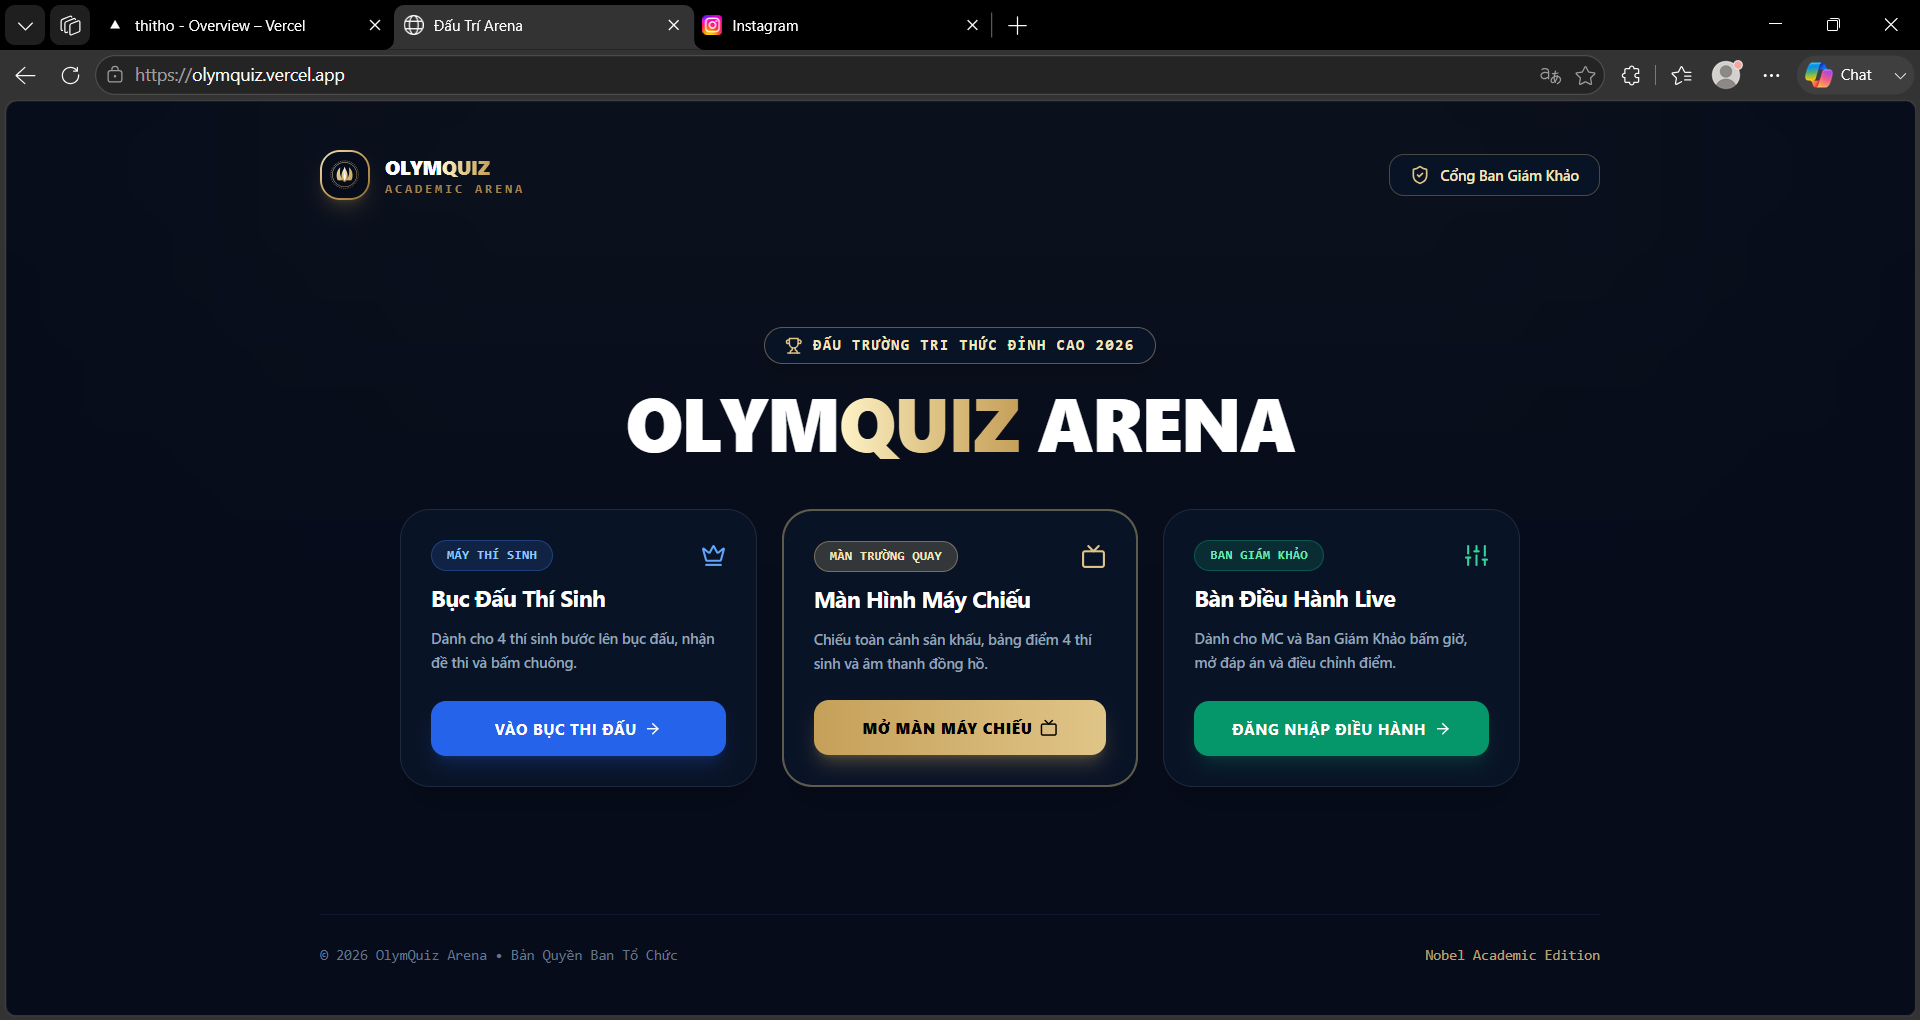
\includegraphics[width=0.96\textwidth]{screenshots/13_admin_live.png}
\end{center}

\vspace{0.2cm}
\noindent\textbf{Bảng Phím Tắt Tiện Lợi Cho Giám Khảo:}\\
\begin{tabularx}{\textwidth}{l l X}
\toprule
\textbf{Phím Tắt} & \textbf{Chức Năng} & \textbf{Hành Động Nhanh} \\
\midrule
\textbf{Space} & Bắt Đầu / Tạm Dừng & Chạy hoặc dừng đếm ngược thời gian câu hỏi. \\
\textbf{L} & Khóa Nộp Bài & Khóa không cho thí sinh bấm nộp nữa. \\
\textbf{G} & Chấm Điểm & Tự động kiểm tra đúng/sai và cộng điểm tức thì. \\
\textbf{R} & Reset Đồng Hồ & Trả thời gian về ban đầu và xóa bài nộp cũ của câu. \\
\bottomrule
\end{tabularx}

\newpage

% ============================================================
% MÀN HÌNH 5: SLIDE GIỚI THIỆU THÍ SINH
% ============================================================
\noindent{\Large\bfseries\color{primary} MÀN HÌNH 5: SLIDE GIỚI THIỆU 4 THÍ SINH XUẤT SẮC}\\[0.1cm]
\noindent\textit{Màn hình Máy Chiếu Hội Trường (\texttt{/display})}\\[0.2cm]
\textbf{Mục đích}: Chiếu toàn cảnh 4 Card thí sinh trang trọng trước trận đấu để MC giới thiệu từng bạn bước lên sân khấu.
\begin{itemize}[leftmargin=*,itemsep=2pt]
    \item Hiển thị số máy (MÁY 1, 2, 3, 4), Họ tên, Đơn vị đại diện và điểm số khởi đầu.
\end{itemize}

\begin{center}
    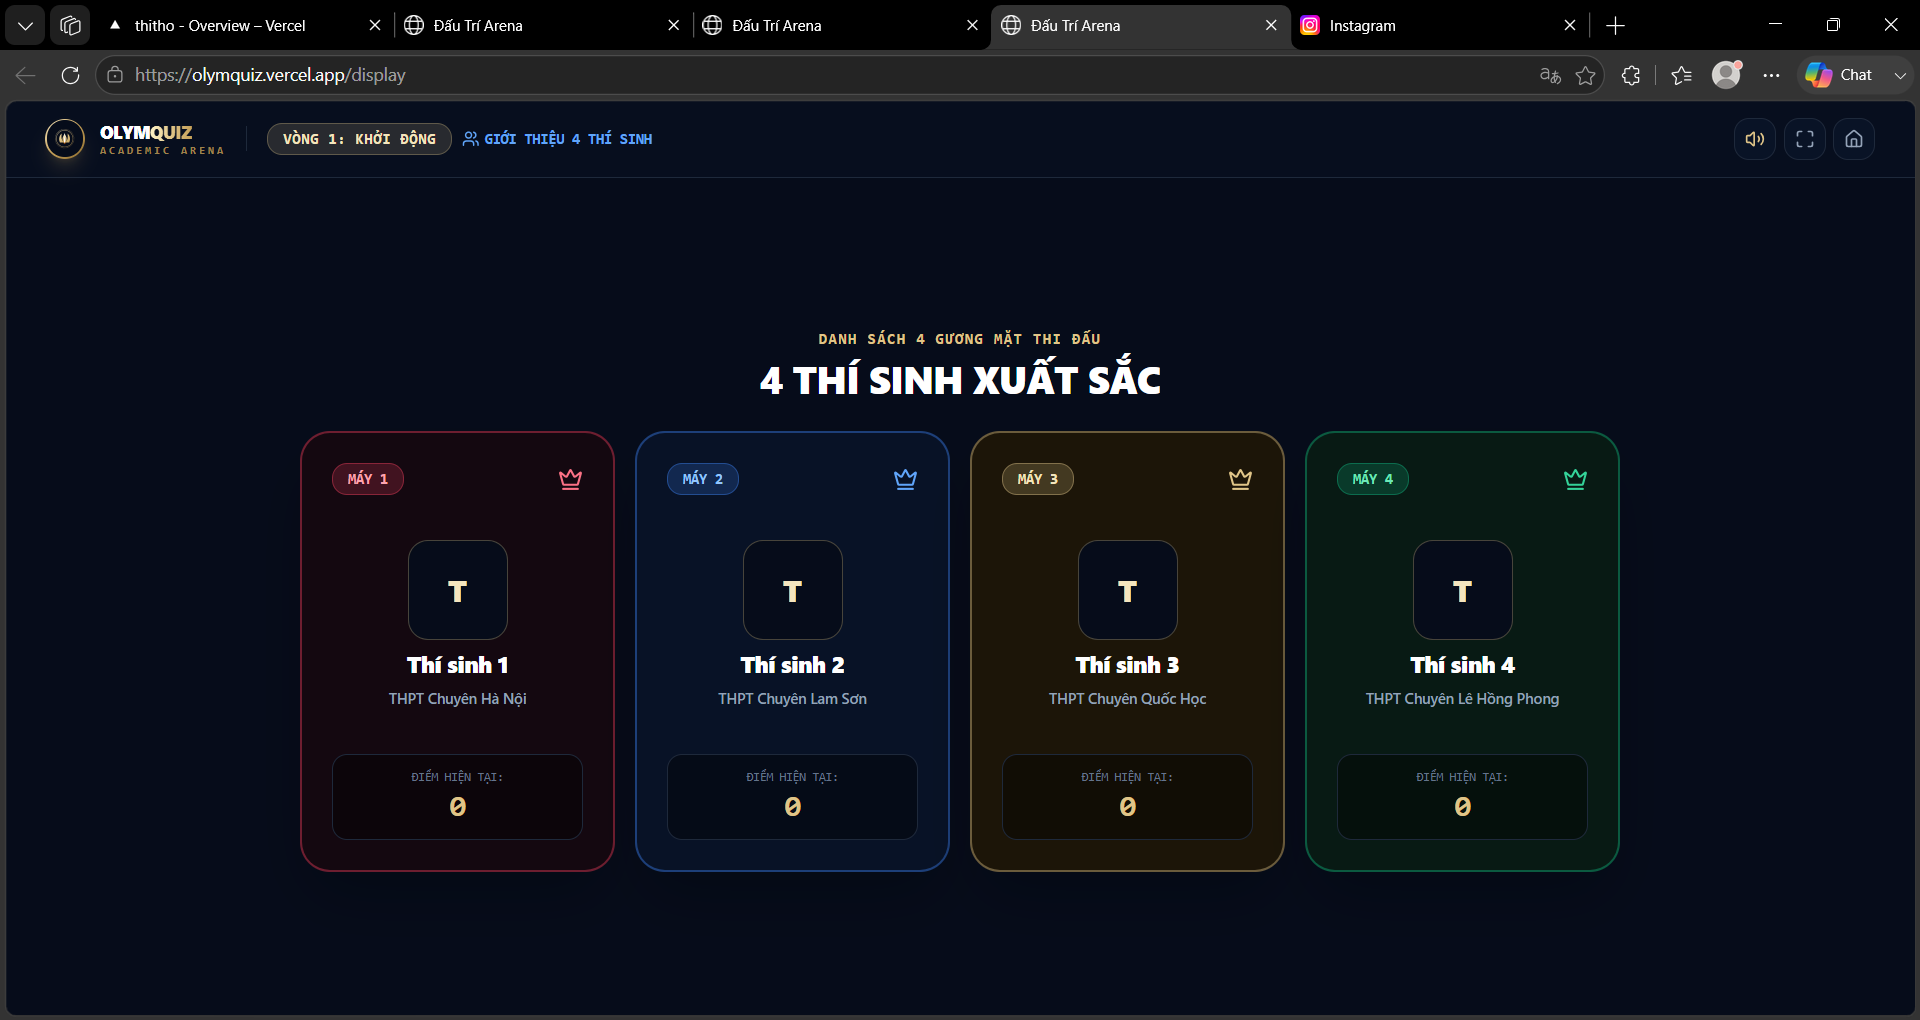
\includegraphics[width=0.96\textwidth]{screenshots/04_display_intro.png}
\end{center}

\vspace{0.4cm}

% ============================================================
% MÀN HÌNH 6: SLIDE THỂ LỆ TỔNG QUAN 4 VÒNG
% ============================================================
\noindent{\Large\bfseries\color{primary} MÀN HÌNH 6: SLIDE THỂ LỆ TỔNG QUAN 4 VÒNG ĐẤU}\\[0.1cm]
\noindent\textit{Màn hình Máy Chiếu Hội Trường (\texttt{/display})}\\[0.2cm]
\textbf{Mục đích}: Giúp MC phổ biến format thi đấu tổng thể cho toàn thể hội trường.
\begin{itemize}[leftmargin=*,itemsep=2pt]
    \item Hiển thị 4 thẻ thể lệ tóm tắt: \textbf{Khởi Động} (15s/câu, +10đ) $\rightarrow$ \textbf{VCNV} (4 hàng ngang, từ khóa chính) $\rightarrow$ \textbf{Tăng Tốc} (10s-20s-30s-40s) $\rightarrow$ \textbf{Về Đích} (Gói câu hỏi, Sao hy vọng, Cướp điểm).
\end{itemize}

\begin{center}
    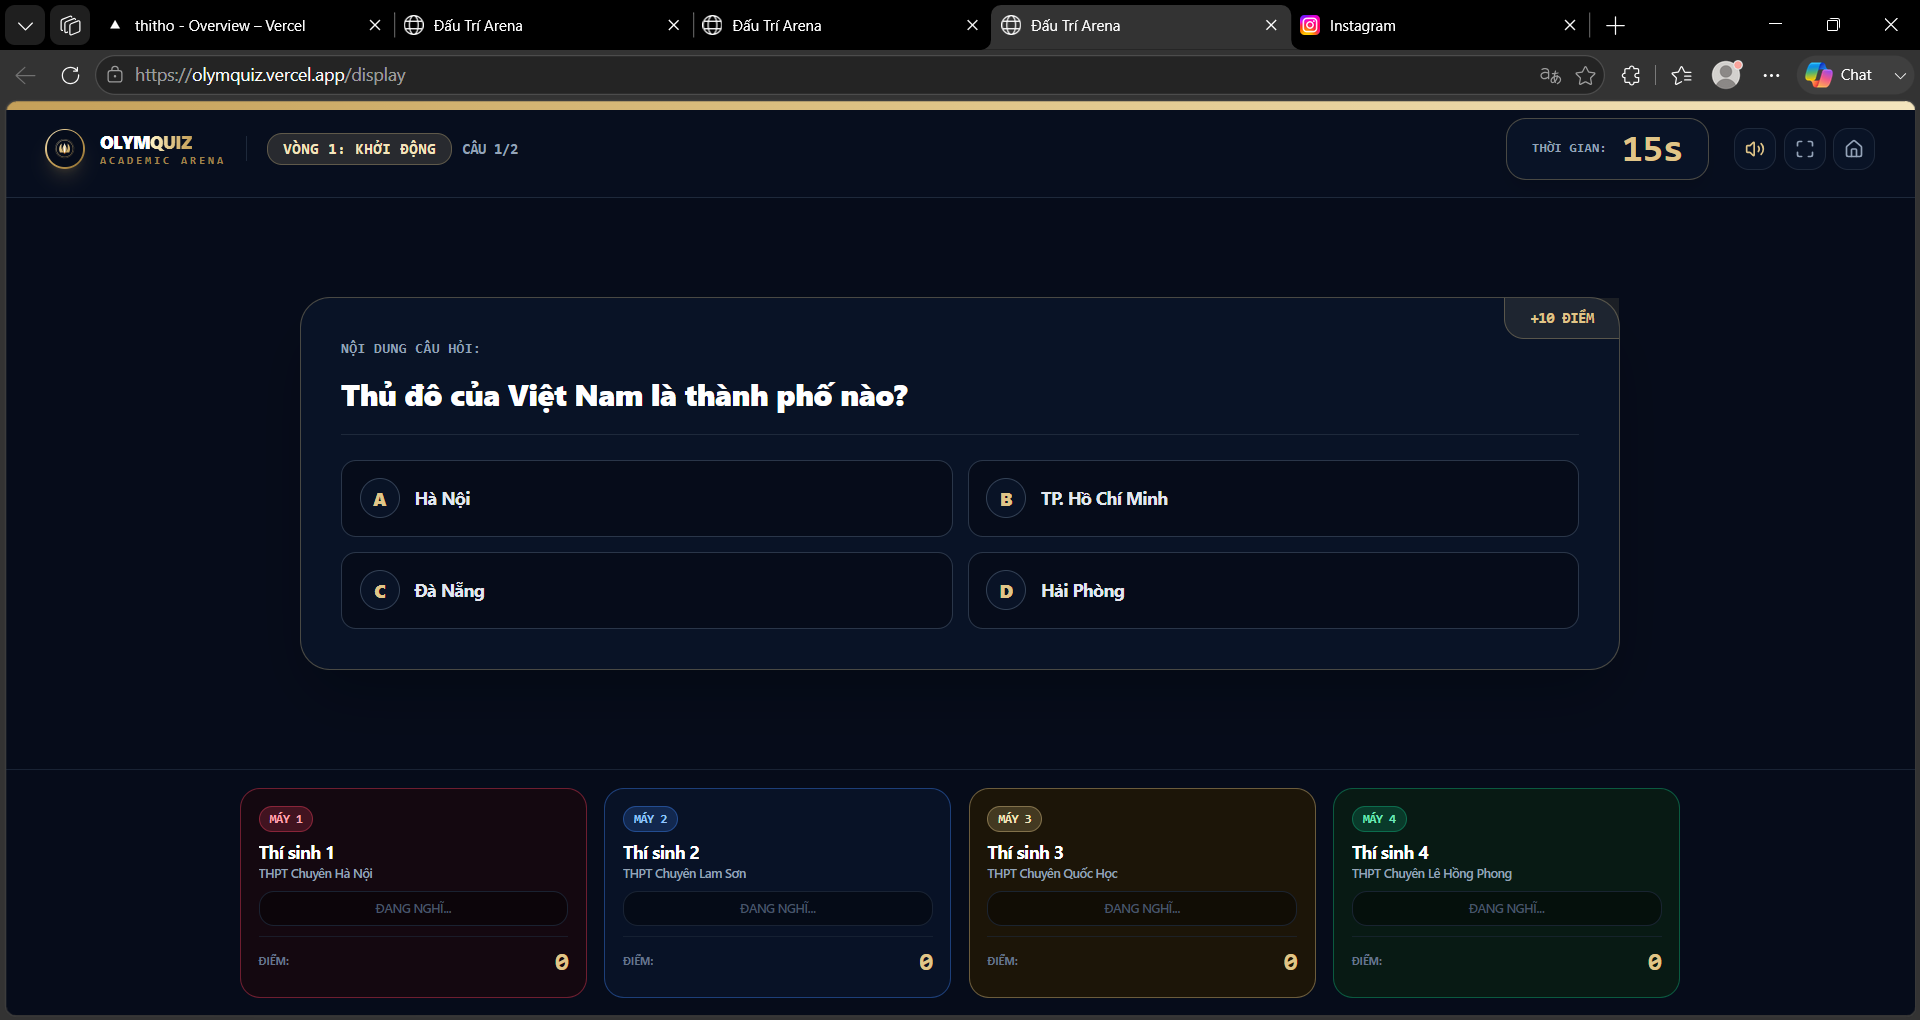
\includegraphics[width=0.96\textwidth]{screenshots/05_display_rules_all.png}
\end{center}

\newpage

% ============================================================
% MÀN HÌNH 7: SLIDE THỂ LỆ VÒNG 1
% ============================================================
\noindent{\Large\bfseries\color{primary} MÀN HÌNH 7: SLIDE CHI TIẾT THỂ LỆ VÒNG 1 (KHỞI ĐỘNG)}\\[0.1cm]
\noindent\textit{Màn hình Máy Chiếu Hội Trường (\texttt{/display})}\\[0.2cm]
\textbf{Mục đích}: Chiếu thể lệ chi tiết của Vòng 1 trước khi bắt đầu câu hỏi đầu tiên.
\begin{itemize}[leftmargin=*,itemsep=2pt]
    \item Thời gian làm bài: 15 giây / câu hỏi trắc nghiệm 4 phương án A, B, C, D.
    \item Cơ chế tính điểm: Trả lời đúng được +10 Điểm. Trả lời sai không bị trừ điểm.
\end{itemize}

\begin{center}
    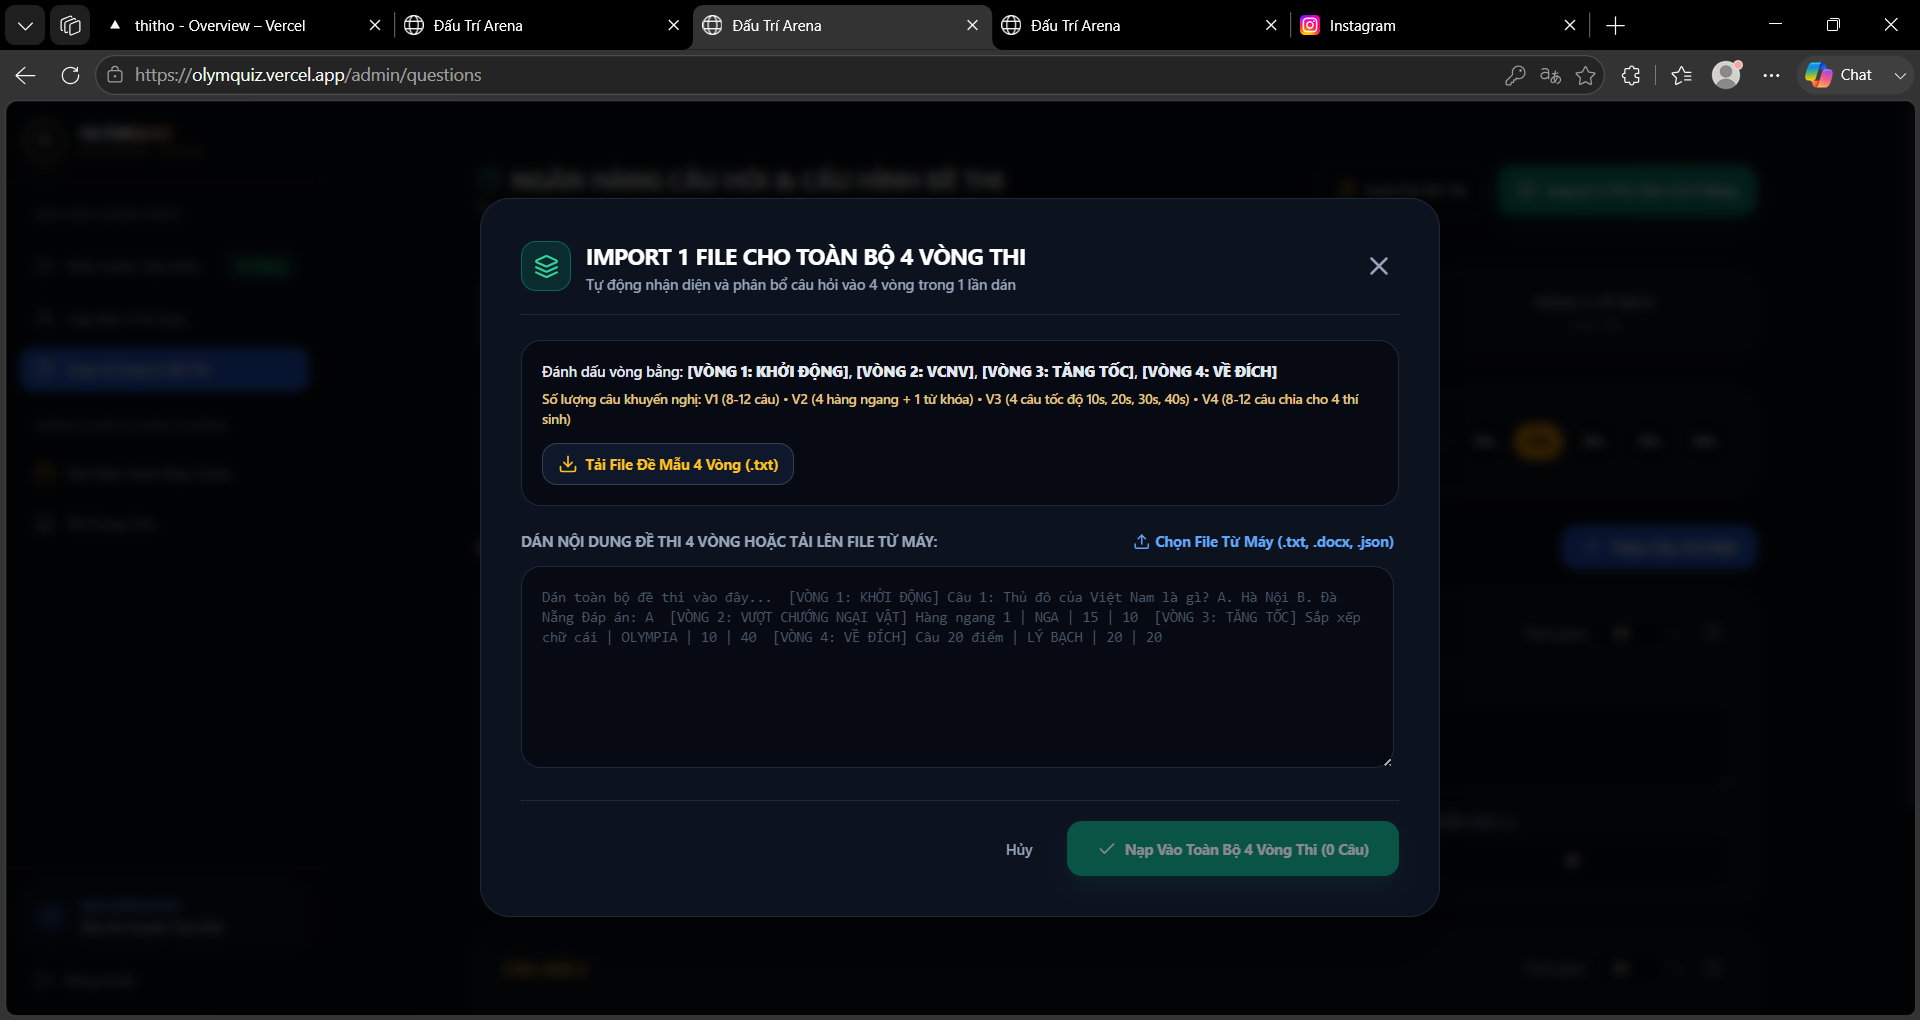
\includegraphics[width=0.96\textwidth]{screenshots/06_display_rule_r1.png}
\end{center}

\vspace{0.4cm}

% ============================================================
% MÀN HÌNH 8: SLIDE THỂ LỆ VÒNG 2
% ============================================================
\noindent{\Large\bfseries\color{primary} MÀN HÌNH 8: SLIDE CHI TIẾT THỂ LỆ VÒNG 2 (VƯỢT CHƯỚNG NGẠI VẬT)}\\[0.1cm]
\noindent\textit{Màn hình Máy Chiếu Hội Trường (\texttt{/display})}\\[0.2cm]
\textbf{Mục đích}: Chiếu luật giải mã 4 hàng ngang và quy định bấm chuông trả lời từ khóa chính.
\begin{itemize}[leftmargin=*,itemsep=2pt]
    \item Mỗi câu hàng ngang đúng được +10 Điểm kèm gợi ý số lượng chữ cái.
    \item Bấm chuông trả lời Chướng ngại vật: +60đ (sau hàng 1), +40đ (sau hàng 2), +20đ (sau hàng 3). Trả lời sai bị loại khỏi vòng.
\end{itemize}

\begin{center}
    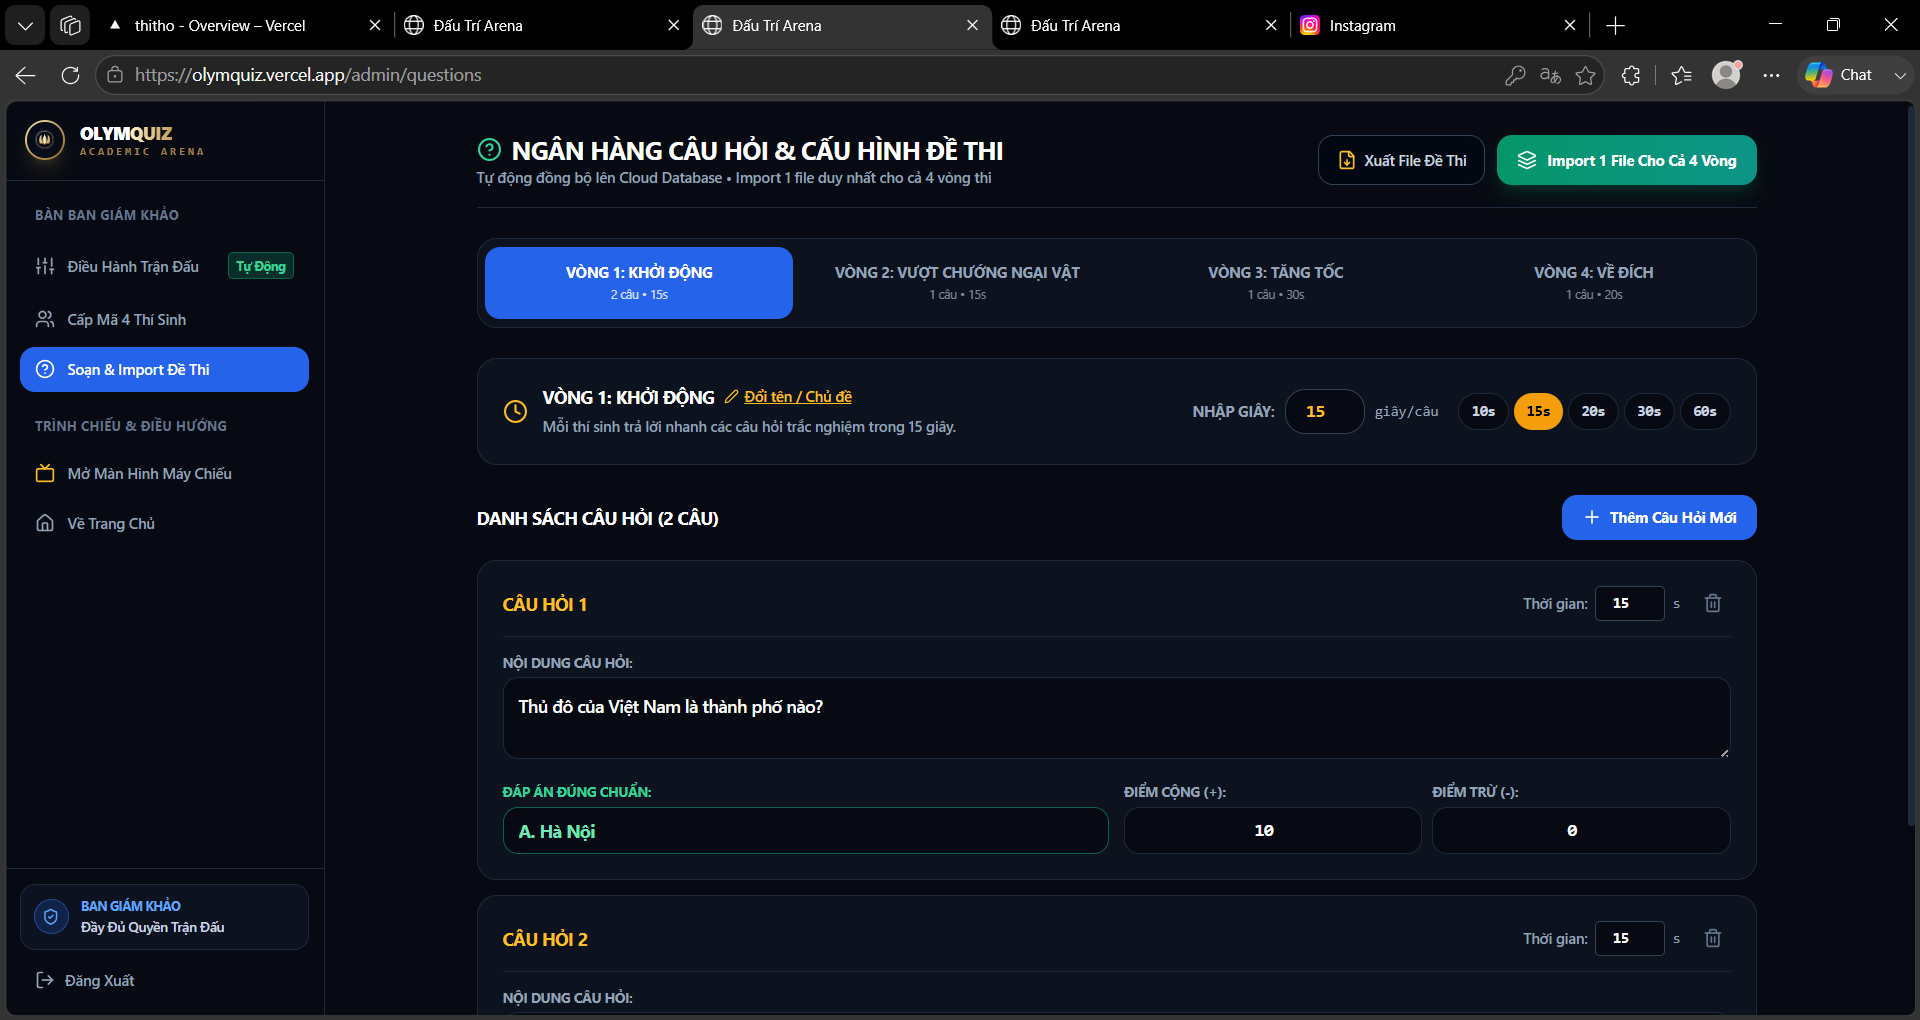
\includegraphics[width=0.96\textwidth]{screenshots/07_display_rule_r2.png}
\end{center}

\newpage

% ============================================================
% MÀN HÌNH 9: SLIDE THỂ LỆ VÒNG 3
% ============================================================
\noindent{\Large\bfseries\color{primary} MÀN HÌNH 9: SLIDE CHI TIẾT THỂ LỆ VÒNG 3 (TĂNG TỐC)}\\[0.1cm]
\noindent\textit{Màn hình Máy Chiếu Hội Trường (\texttt{/display})}\\[0.2cm]
\textbf{Mục đích}: Chiếu luật cuộc đua tốc độ tính bằng mili-giây.
\begin{itemize}[leftmargin=*,itemsep=2pt]
    \item 4 mốc thời gian tăng dần: 10 giây (câu 1) $\rightarrow$ 20 giây (câu 2) $\rightarrow$ 30 giây (câu 3) $\rightarrow$ 40 giây (câu 4).
    \item Thang điểm cộng theo tốc độ nộp: Nhanh nhất (+40đ) $\rightarrow$ Nhì (+30đ) $\rightarrow$ Ba (+20đ) $\rightarrow$ Tư (+10đ).
\end{itemize}

\begin{center}
    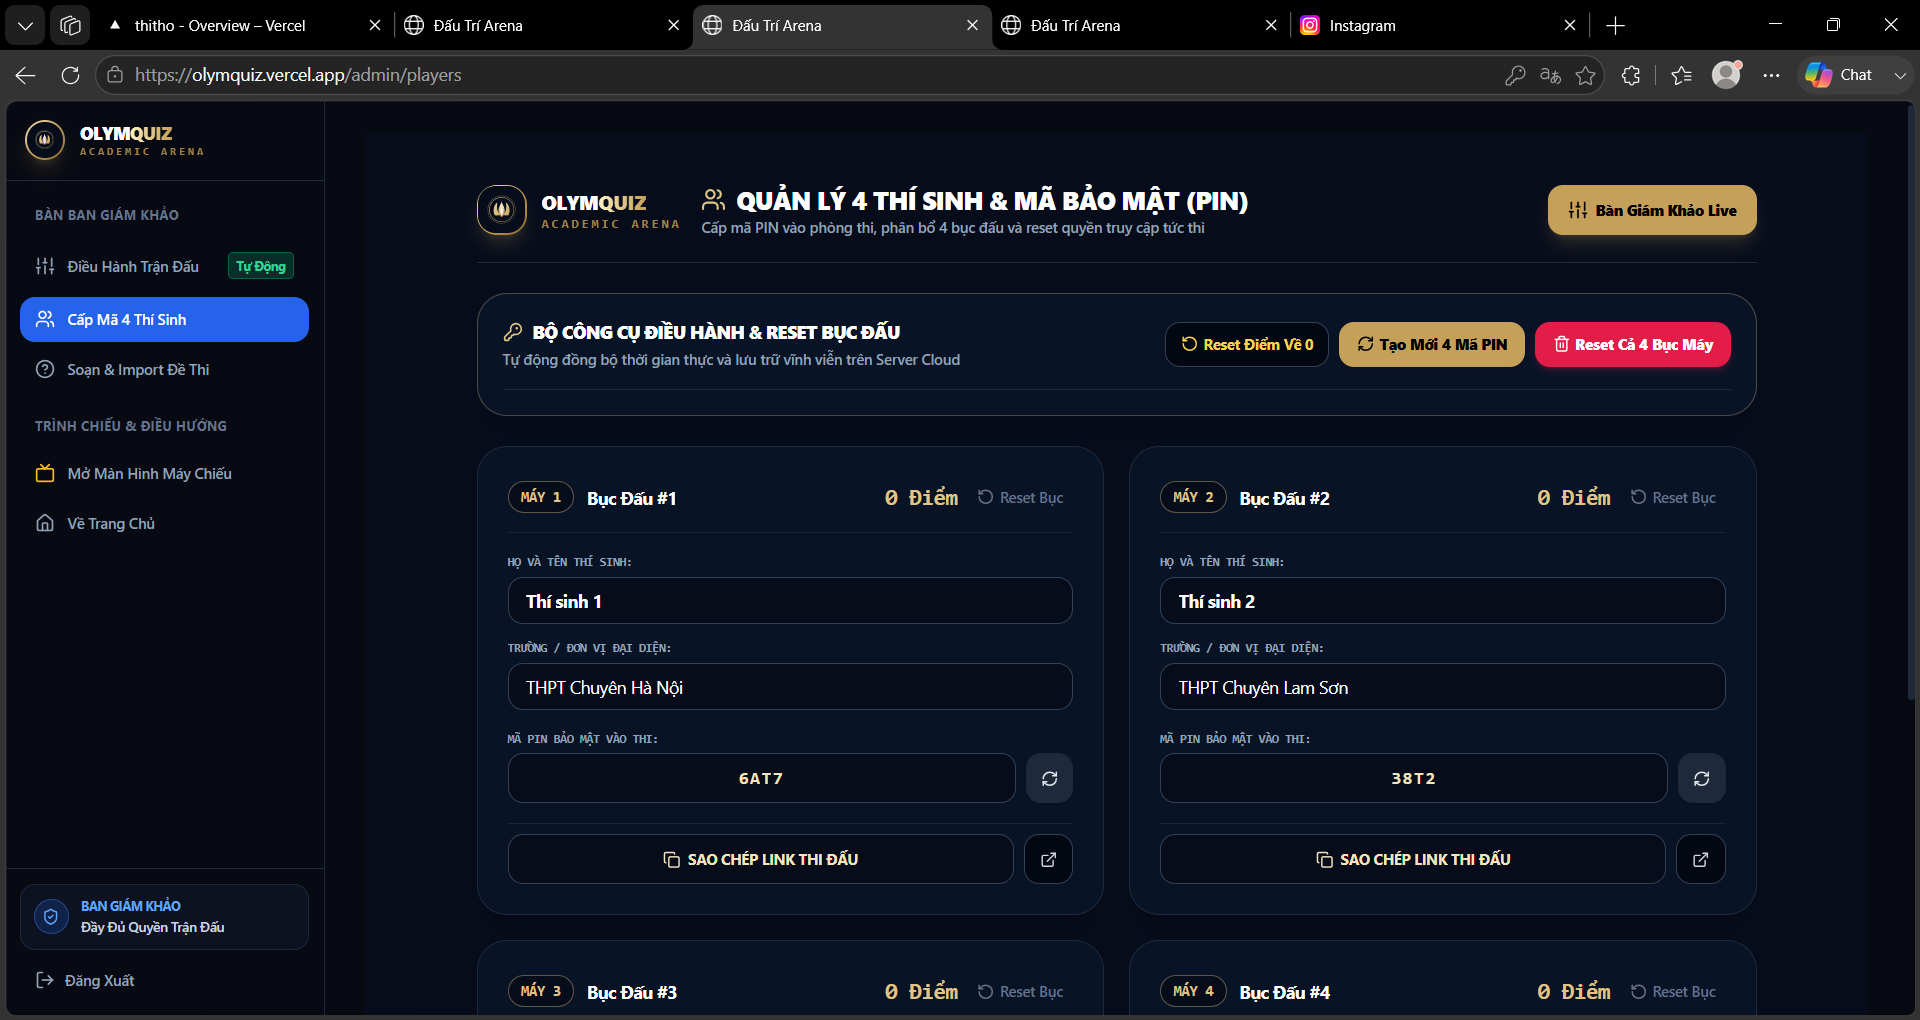
\includegraphics[width=0.96\textwidth]{screenshots/08_display_rule_r3.png}
\end{center}

\vspace{0.4cm}

% ============================================================
% MÀN HÌNH 10: SLIDE THỂ LỆ VÒNG 4
% ============================================================
\noindent{\Large\bfseries\color{primary} MÀN HÌNH 10: SLIDE CHI TIẾT THỂ LỆ VÒNG 4 (VỀ ĐÍCH)}\\[0.1cm]
\noindent\textit{Màn hình Máy Chiếu Hội Trường (\texttt{/display})}\\[0.2cm]
\textbf{Mục đích}: Chiếu luật gói câu hỏi 20đ/30đ, Ngôi Sao Hy Vọng và Chuông cướp điểm.
\begin{itemize}[leftmargin=*,itemsep=2pt]
    \item Mỗi bạn có 1 lượt thi chính. Được quyền đặt \textbf{Ngôi Sao Hy Vọng} (+x2 điểm nếu đúng, -50\% nếu sai).
    \item Nếu thí sinh chính trả lời sai, 3 bạn còn lại được quyền Bấm Chuông Cướp Điểm.
\end{itemize}

\begin{center}
    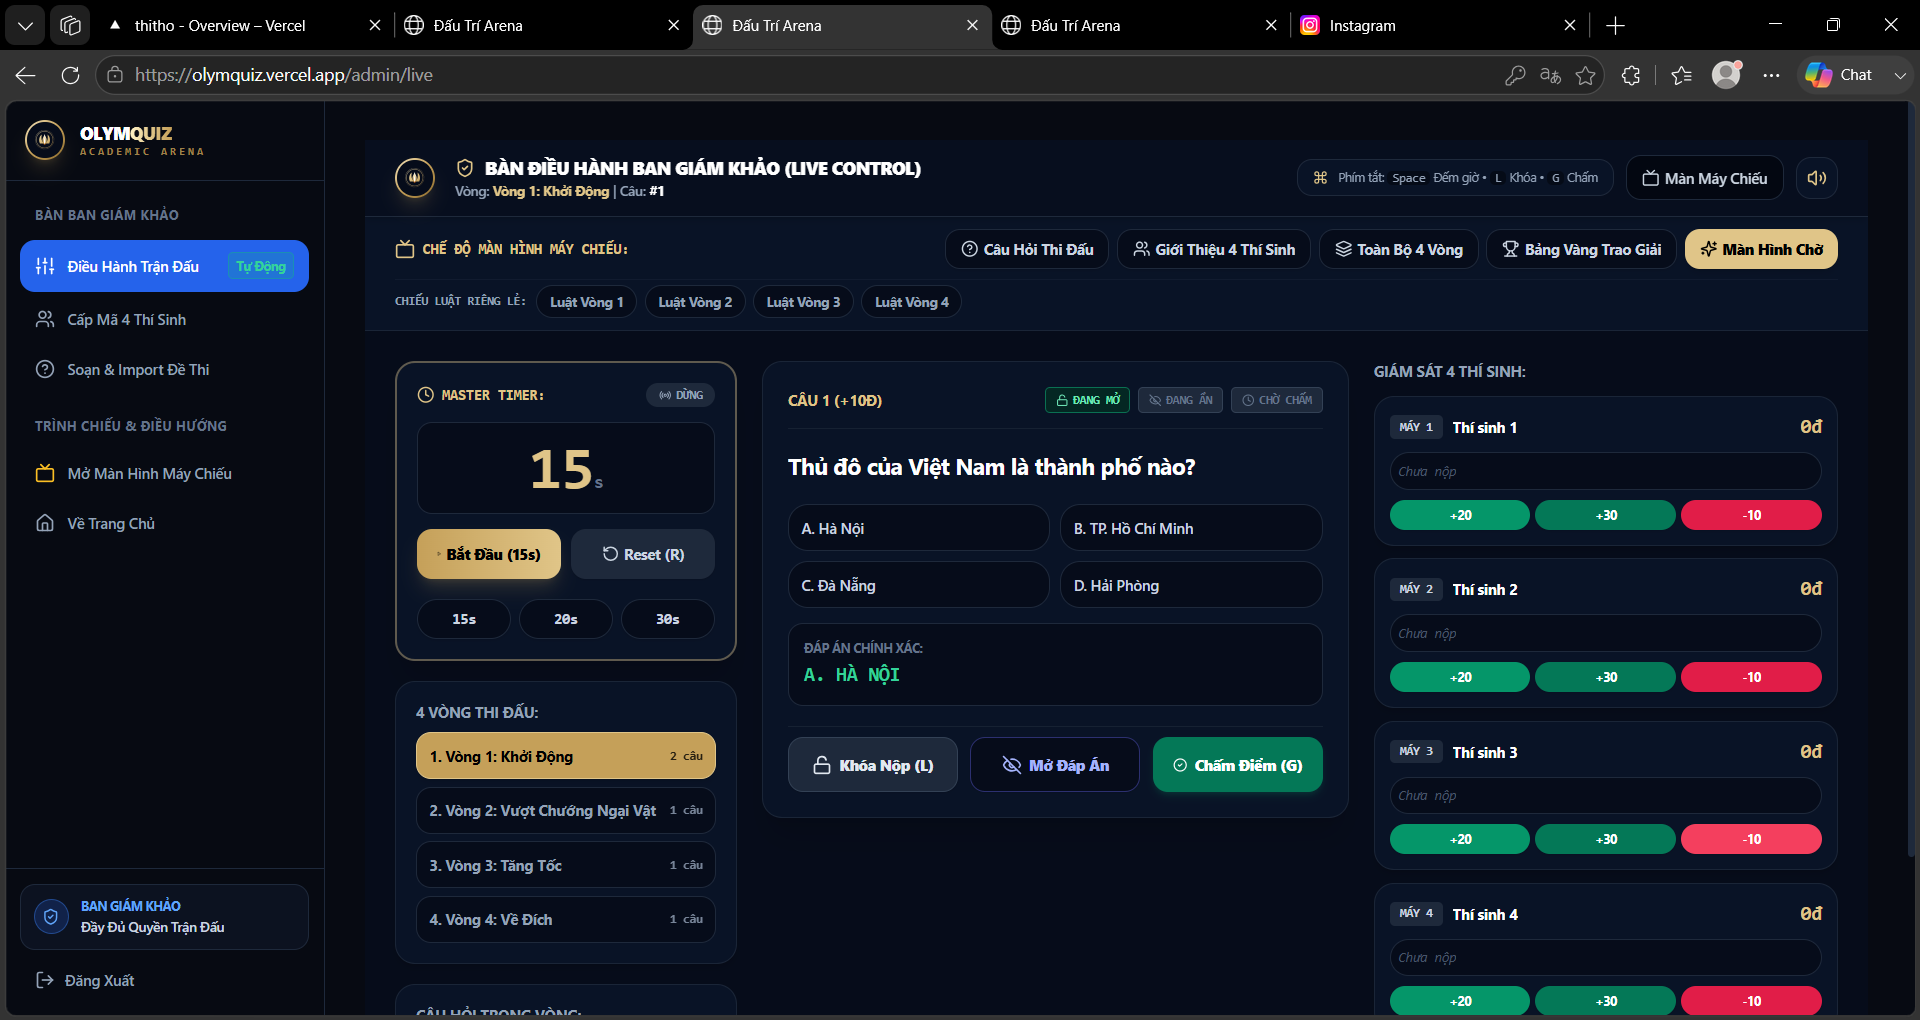
\includegraphics[width=0.96\textwidth]{screenshots/09_display_rule_r4.png}
\end{center}

\newpage

% ============================================================
% MÀN HÌNH 11: MÁY CHIẾU THI ĐẤU CÂU 1
% ============================================================
\noindent{\Large\bfseries\color{primary} MÀN HÌNH 11: MÀN MÁY CHIẾU CÂU HỎI 1 (ĐÃ CÔNG BỐ ĐÁP ÁN)}\\[0.1cm]
\noindent\textit{Màn hình Máy Chiếu Hội Trường (\texttt{/display})}\\[0.2cm]
\textbf{Mục đích}: Hiển thị kết quả công khai và minh bạch cho toàn bộ khán phòng theo dõi.
\begin{itemize}[leftmargin=*,itemsep=2pt]
    \item \textbf{Phương Án Đúng (A. Hà Nội)}: Tự động phát sáng viền xanh ngọc bích nổi bật.
    \item \textbf{4 Bục Điểm Dưới Chân}: Tự động hiện đáp án của từng bạn kèm dấu tick xanh cho câu đúng và dấu nhân đỏ cho câu sai.
\end{itemize}

\begin{center}
    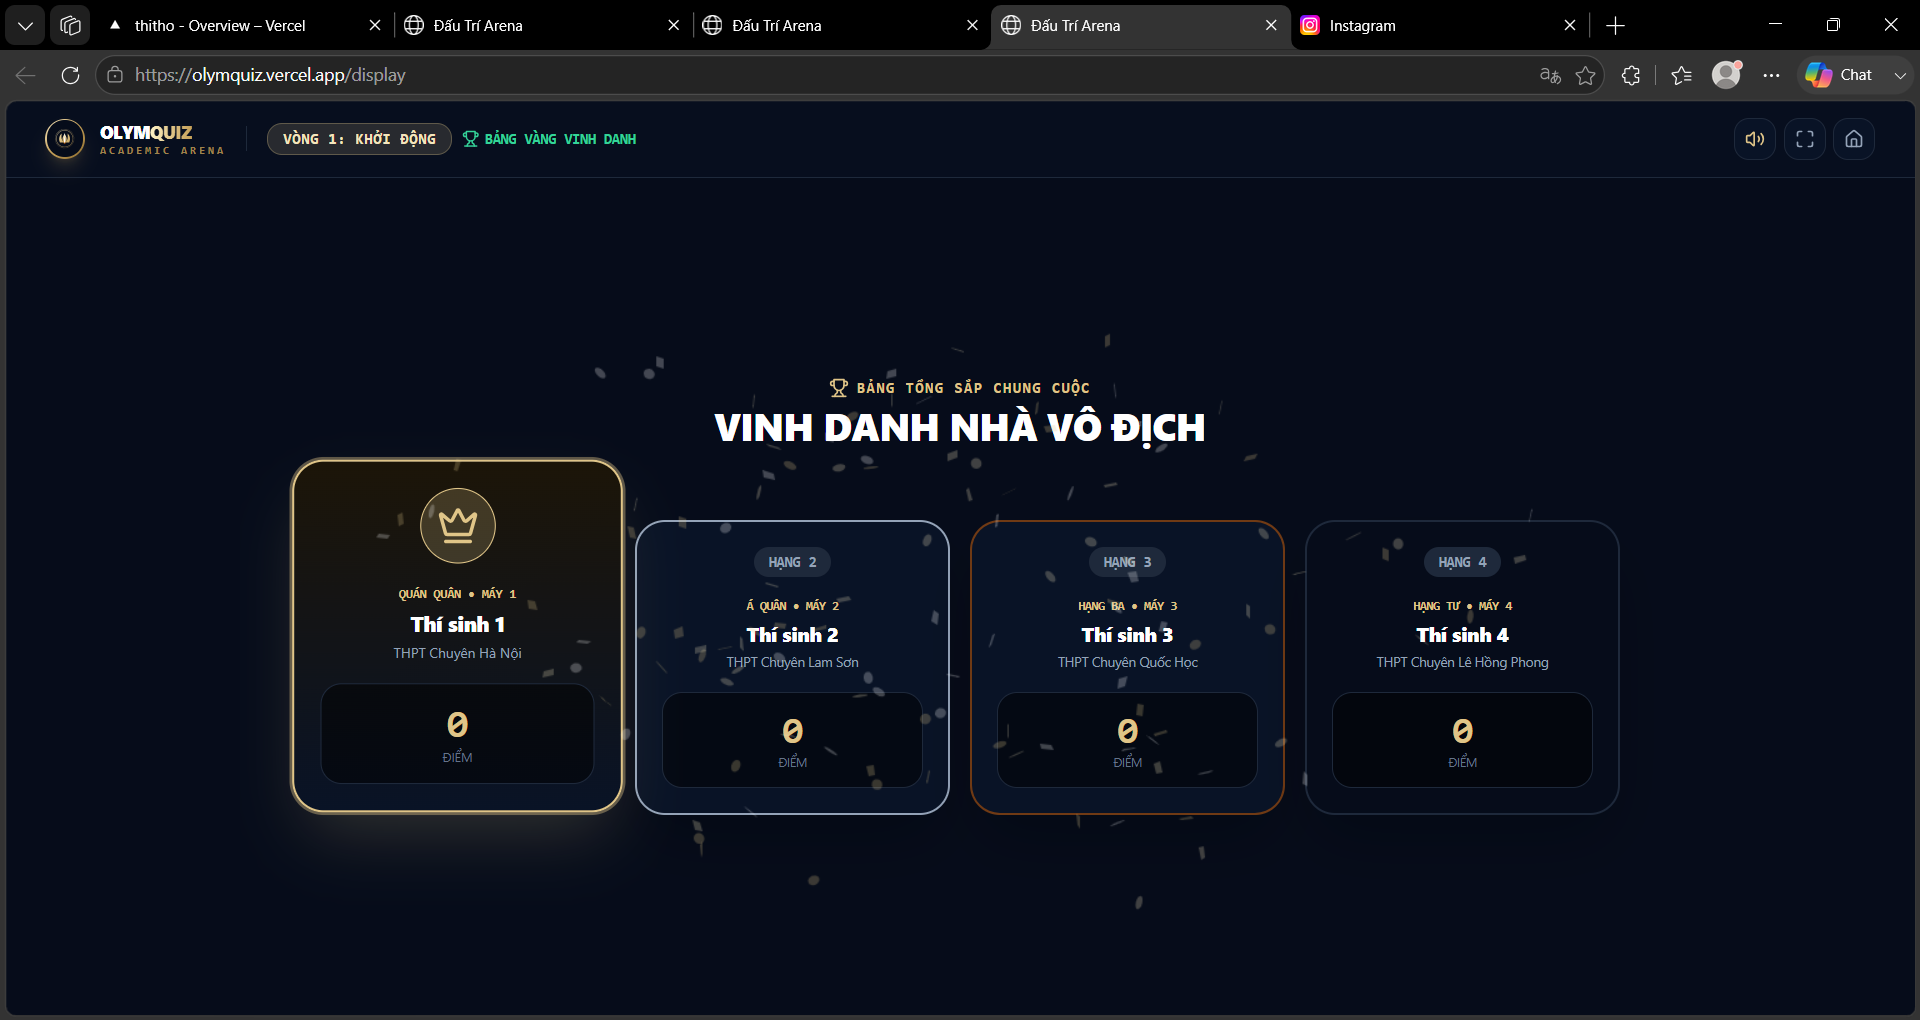
\includegraphics[width=0.96\textwidth]{screenshots/02_display_q1.png}
\end{center}

\vspace{0.4cm}

% ============================================================
% MÀN HÌNH 12: MÁY CHIẾU THI ĐẤU CÂU 2
% ============================================================
\noindent{\Large\bfseries\color{primary} MÀN HÌNH 12: MÀN MÁY CHIẾU CÂU HỎI 2 (ĐANG TRONG THỜI GIAN ĐẾM LÙI)}\\[0.1cm]
\noindent\textit{Màn hình Máy Chiếu Hội Trường (\texttt{/display})}\\[0.2cm]
\textbf{Mục đích}: Giao diện thi đấu trực tiếp khi đồng hồ đang chạy.
\begin{itemize}[leftmargin=*,itemsep=2pt]
    \item \textbf{Thanh Laser Timer trên cùng}: Chạy lùi theo thời gian thực (đổi màu đỏ khi còn dưới 3 giây).
    \item \textbf{Đồng hồ LED to}: Hiển thị số giây còn lại sắc nét ở góc phải trên.
\end{itemize}

\begin{center}
    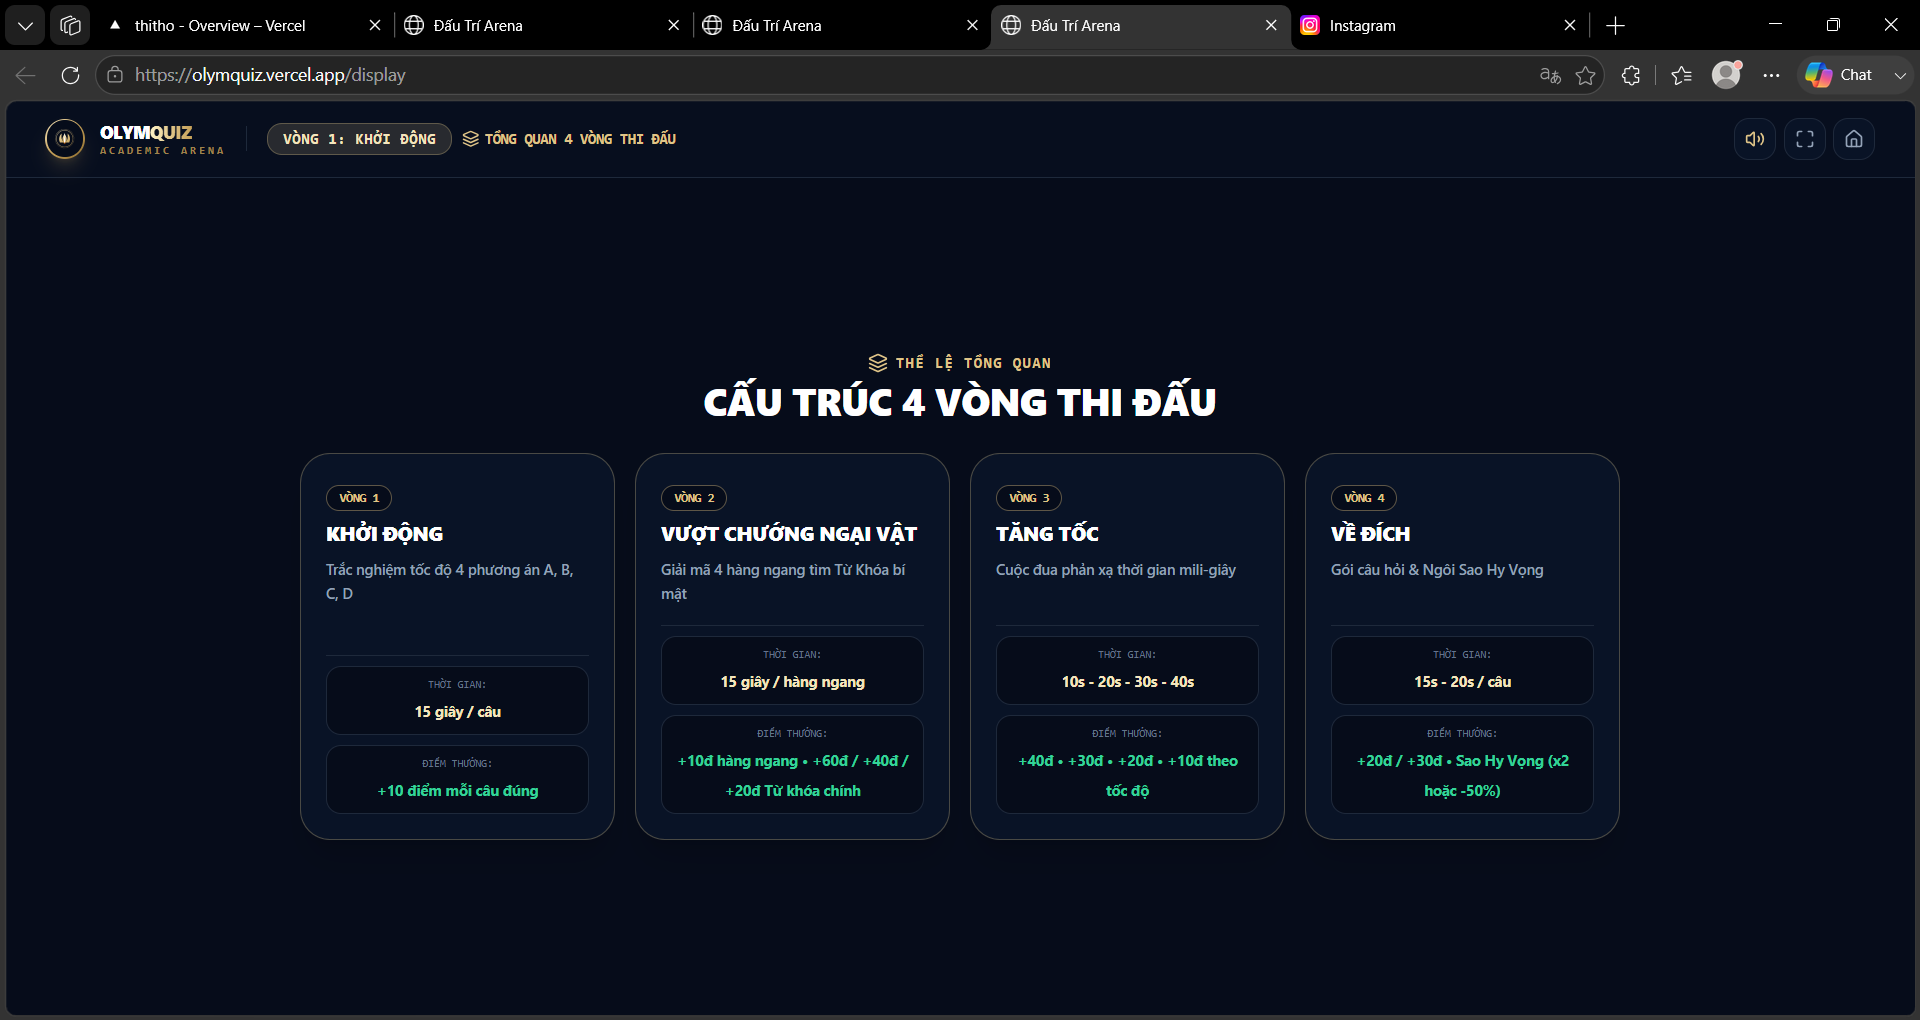
\includegraphics[width=0.96\textwidth]{screenshots/03_display_q2.png}
\end{center}

\newpage

% ============================================================
% MÀN HÌNH 13: BẢNG VÀNG TRAO GIẢI
% ============================================================
\noindent{\Large\bfseries\color{primary} MÀN HÌNH 13: SLIDE BẢNG VÀNG VINH DANH \& TRAO GIẢI}\\[0.1cm]
\noindent\textit{Màn hình Máy Chiếu Hội Trường (\texttt{/display})}\\[0.2cm]
\textbf{Mục đích}: Màn hình bế mạc vinh danh nhà vô địch và trao giải chung cuộc.
\begin{itemize}[leftmargin=*,itemsep=2pt]
    \item Hệ thống tự động xếp thứ hạng \textbf{Quán Quân -- Á Quân -- Hạng Ba -- Hạng Tư} dựa trên tổng điểm.
    \item Tự động kích hoạt hiệu ứng \textbf{Pháo Hoa Confetti rực rỡ} và biểu tượng Vương miện Hoàng kim Nobel!
\end{itemize}

\begin{center}
    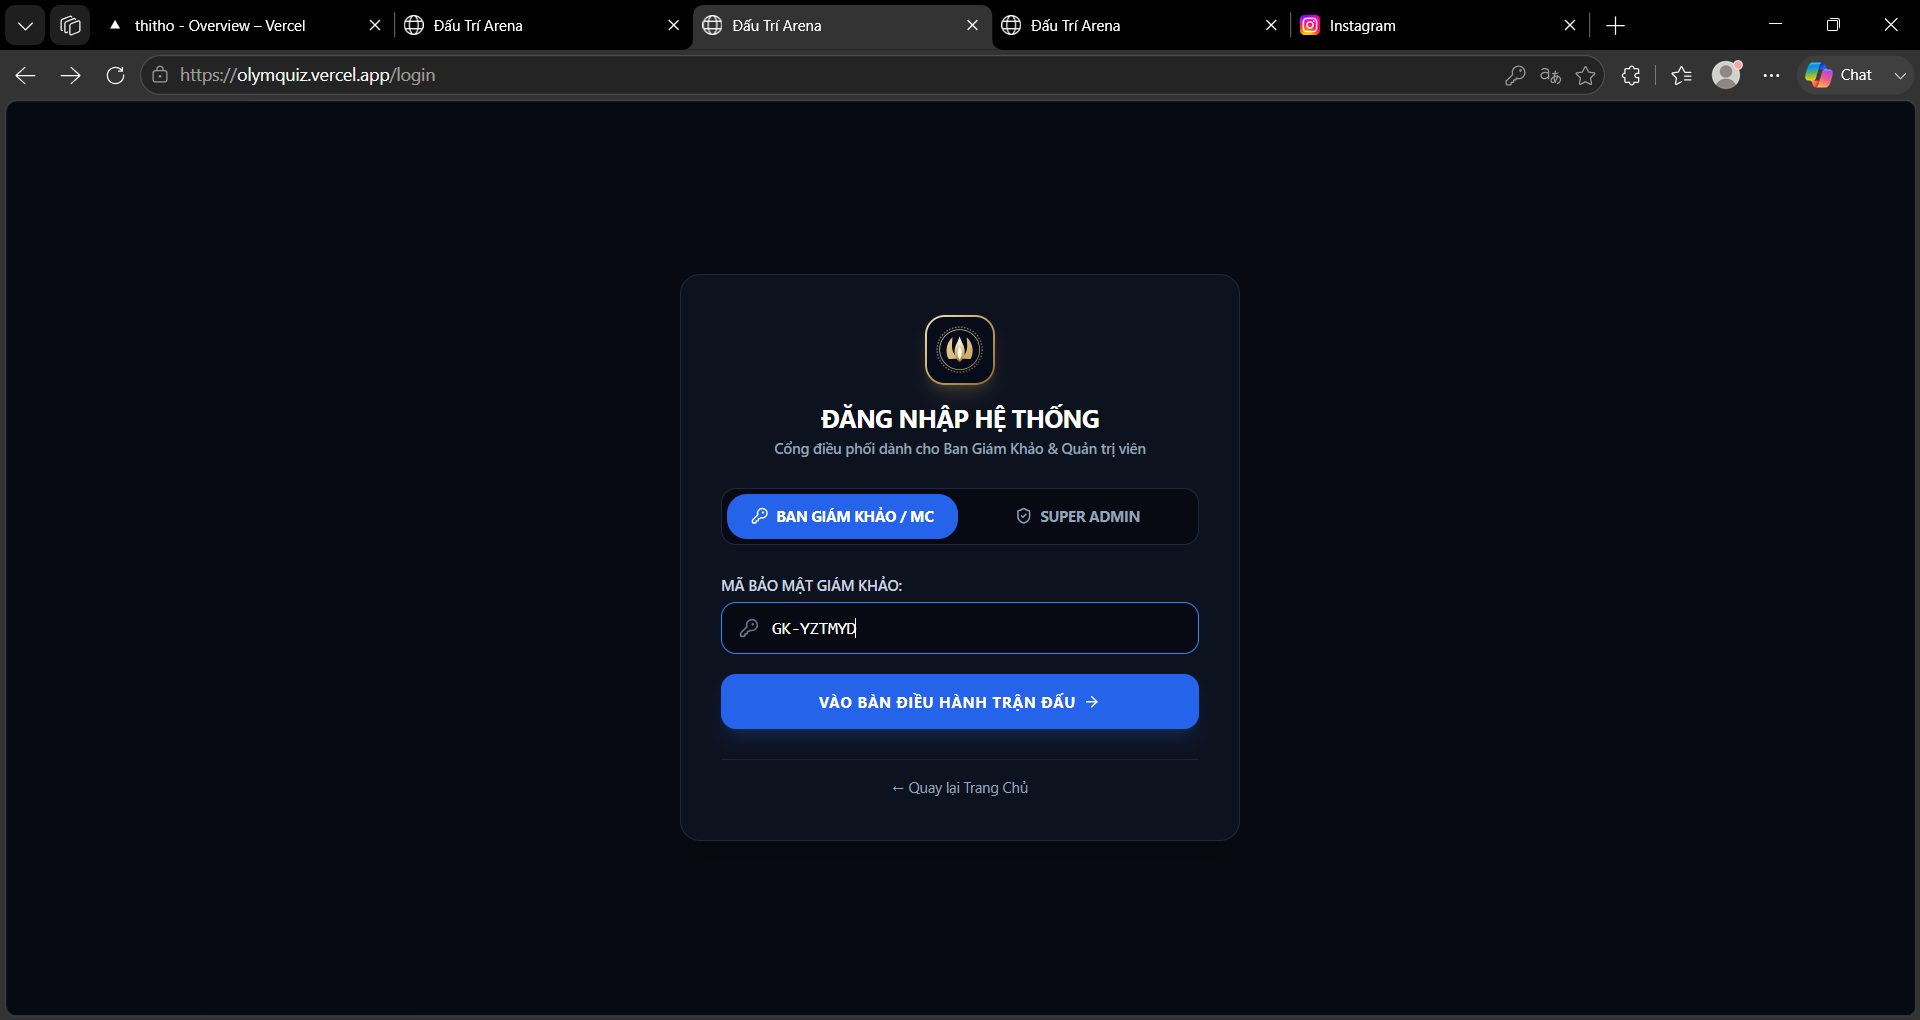
\includegraphics[width=0.96\textwidth]{screenshots/10_display_leaderboard.png}
\end{center}

\vspace{0.8cm}
\begin{center}
    \rule{\textwidth}{1.5pt}\\[0.3cm]
    {\Large\bfseries\color{primary} CHÚC BẠN VÀ NGƯỜI YÊU TỔ CHỨC BUỔI THI ĐẤU THÀNH CÔNG RỰC RỠ!}\\[0.2cm]
    {\small Bản quyền © 2026 OlymQuiz Academic Arena -- Website: \texttt{https://olymquiz.vercel.app}}
\end{center}

\end{document}
